\documentclass[10pt, a4paper]{article}
\usepackage[utf8]{inputenc}
\usepackage{pdflscape}
\usepackage{amssymb}
% \usepackage[margin=3cm]{geometry}
\usepackage{graphicx}
\usepackage{oz}
\usepackage{array,multirow,makecell}
\setcellgapes{1pt}
\usepackage[top=4cm,bottom=4cm,left=3cm,right=3cm]{geometry} %marges
\newcolumntype{R}[1]{>{\raggedleft\arraybackslash }b{#1}}
\newcolumntype{L}[1]{>{\raggedright\arraybackslash }b{#1}}
\newcolumntype{C}[1]{>{\centering\arraybackslash }b{#1}}

\title{Analyse Projet BDD}
\date{}
\begin{document}


\maketitle
\tableofcontents
\newpage

\section{Analyse du problème}
\subsection{Hypothèses}
Pour la conception, nous avons fait les choix suivants :
\begin{enumerate}
    \item Le statut des commandes n'est pas dans l'entité mère COMMANDES 
mais dans ses sous-entités afin d'éviter d'avoir des statuts non cohérents 
pour un type de commande donné.
    \item Nous avons rajouté le statut "terminée" qui indique qu'une 
commande a effectivement été effectuée et que l'on peut donner un 
évaluation
\end{enumerate}

Nous sommes arrivés avec les contraintes suivantes :
\begin{landscape}
\subsection{Contraintes}

\begin{center}
\[
\begin{tabular}{|C{5cm}|C{5cm}|C{5cm}|C{5cm} |}

\hline
DF& C. Valeurs 
& C. Contextuelles & C. Multiplicité\\
\hline

RMail $\rightarrow$ RNom, RNumero, RAdresse, Places, 
Presentation, RNote & RType $\in$ \{livraison, emporter, place\} & $\sum 
\mbox{nbPers}  \le \mbox{Places} $ pour un restaurant et ses commandes 
associées & RMail $\twoheadrightarrow$ JourPlage\\

 & Places $> 0$ & $\mbox{Ext(CEId)} \cap \mbox{Ext(CPId)} \cap 
\mbox{Ext(CLId)} = \emptyset $ &  RMail  $\twoheadrightarrow$ 
TypeCommande\\ 
 
 & RNote $\in  [0,5] $ &  $\mbox{Ext(CEId)} \cup \mbox{Ext(CPId)} \cup 
\mbox{Ext(CLId)} = \mbox{Ext(CId)}$ & RMail $\twoheadrightarrow$ PId\\
\cline{1-2}

(PId, Restaurant) $\rightarrow$ PNom, PDescription, PPrix & PPrix $>0$ & 
CPArrivee $\in$ JourPlage pour un restaurant et ses commandes associées & 
RMail $\twoheadrightarrow$ CatNom\\
\cline{1-2}

U\_Id $\rightarrow$ UMail, UMdp, UNom, UPrenom, UAdresse && CDate donne JourPlage pour toute commande& (PId, RMail) $\psur$ ANom \\
\cline{1-2}

CId $\rightarrow$ CDate, CPrix & CPrix $>0$ & CDate $\le$ EDate& 
CId $\twoheadrightarrow$ (PId, RMail)\\
\cline{1-2}

CLId $\rightarrow$ CLAdresse, Indications, CLArrivee, CLStatut & 
CLStatut $\in$ \{ attente, validée, en livraison, annuleeC, annuleeR, 
terminee \}&
EId $\Rightarrow$ CId.statut = \{terminee\}
& CId $\rightarrow$ TypeCommande \\ 
\cline{1-2}

CEId $\rightarrow$ CEStatut &
CEStatut $\in$ \{ attente, validée, disponible, annuleeC, annuleeR, terminee \}&  & CId $\rightarrow$ U\_Id\\
\cline{1-2}

CPId $\rightarrow$ NbPers, CPArrivee, CPStatut &
CPStatut $\in$ \{ attente, validée, annuleeC, annuleeR, 
terminee \}&  & CId $\pfun$ 
EId\\

& NbPers $>0$ & & CatNom $\pfun$ CatNom\\
\cline{1-2}

EId $ \rightarrow$ EDate, Avis, ENote & ENote $ \in [0..5] $&
CType $\in$ TypeCommande pour un CId donné et le RMail associé &\\ 
\cline{1-2}

& JourHeure $\in $ \{LM, LS, MM, MS, MeM, MeS, JM, JS, VM, VS, SM, SS, DM, 
DS \} & & \\
\hline

\end{tabular}
\]
\end{center}


\newpage
\subsection{Diagramme Entités/Associations}
On obtient ensuite le diagramme Entité-Relation suivant :
\begin{center}
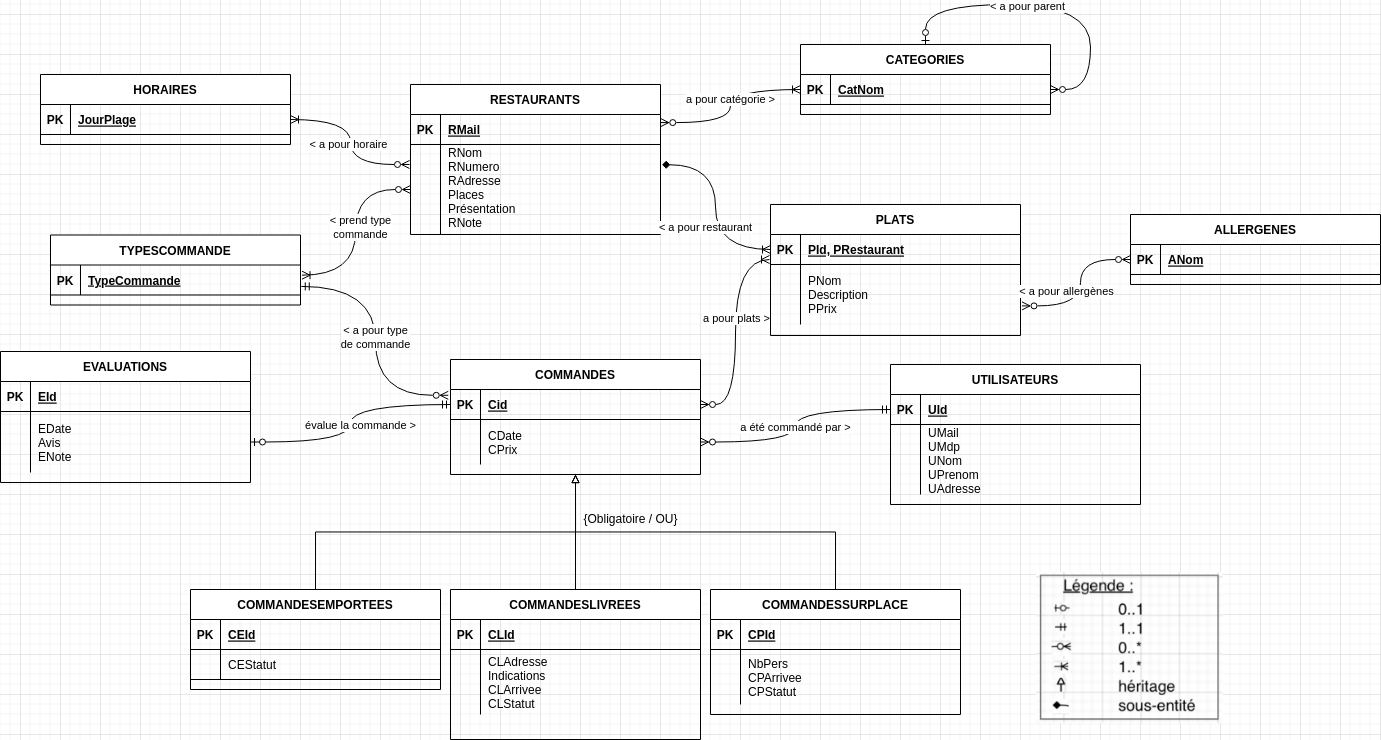
\includegraphics[scale=0.7]{Diagramme_entite_relation.png}\\
\end{center}

\end{landscape}
\section{Modèle Relationnel}
\section{Analyse des fonctionnalités}
\section{Bilan du projet}
\section{Mode d'emploi}

Nous avons développé, comme demandé initialement, un démonstrateur en Java.

Après la panne informatique de l'Ensimag et l'arrêt de l'obligation du démonstrateur, nous avons quand même voulu rendre un démonstrateur fonctionnel, même si toutes les fonctionnalités n'ont pas été introduites. Ainsi, Oracle n'étant pas accessible, nous avons développé la Base de Données en SQLite, en local.

Nous avons alors exporté le démonstrateur dans un \texttt{.jar}. Pour démarrer le démonstrateur, il faut aller dans le dossier Interpréteur et lancer la commande \texttt{java -jar GrenobleEAT.jar}. \\


La navigation dans le navigateur est assez intuitive. L'utilisateur peut naviguer de menu en menu en suivant les instructions demandées. Pour sélectionner les options proposées par  démonstrateur, l'utilisateur devra introduire soit le chiffre correspondant à l'option souhaitée, soit exactement écrirel'option souhaitée. L'application indiquera quand est-ce qu'il faut introduire l'option en chiffre et quand en toutes lettres. \\

Lorsqu'un utilisateur veut réaliser une commande, il peut soit voir la liste des restaurants soit explorer les catégories de l'application.

La liste des restaurants s'affiche dans l'ordre décroissant des évaluations des utilisateurs et dans l'ordre alphabétique des noms. \\

Pour l'exploration des catégories, tout d'abord l'application recommande à l'utilisateur les 3 dernières catégories commandées. Puis, si les catégories ne convainquent pas l'utilisateur ou si simplement l'utilisateur manque de commandes réalisées, nous avons choisi de faire un parcours sous forme d'arbre. Au début, l'application propose des catégories générales, et l'utilisateur peut soit sélectionner la catégorie courante, soit continuer à parcourir les sous-catégories. Puis, l'application montre les restaurants spécialisés dans les catégories choisies. \\

L'utilisateur peut alors choisir les plats qu'il veut dans le restaurant choisi. Une fois qu'il a fini sa sélection, l'utilisateur choisi entre commander en livraison, sur place ou à emporter. L'application demandera alors les informations complémentaires. \\

Pour s'identifier dans l'application, l'utilisateur soit rentrer dans sa session en indiquant son email et mot de passe, soit créer un nouveau compte en introduisant toutes les données nécessaires. Si un utilisateur souhaite demander un effacement de ses données, le demander à l'application dans l'option correspondante. Le compte efface alors toutes les données personnelles, mais existe encore dans l'application même s'il reste non accessible. Ceci permet de garder les évaluations et l'historique des commandes sans que celles-ci soient attribuées à une personne. \\

Finalement, l'utilisateur peut aussi évaluer les commandes réalisées dans le passé. Il pourra voir les commandes réalisées et choisir une note de 0 à 5, ainsi que laisser un commentaire optionnel.
\end{document}


